\section{Factor Analysis} 

  As we have constantly seen, there are specific themes that run between models. In PCA, we have taken some data $x$ in high-dimension $d$ and reduced it to a lower-dimensional orthogonal representation in $\mathbb{R}^k$. In other words, for some sample $x \in \mathbb{R}^{1 \times d}$, the projection onto its component space $x V_k \in \mathbb{R}^{1 \times k}$ is a more parsimonious representation with respect to some other basis vectors. The $v_1, \ldots, v_k$ are new features that are linear combinations of the old vectors. Are they interpretable? In some cases yes and in most cases no, which is why we also call them \textit{latent variables} that live in a \textit{latent space}. 

  Another type of model that encodes covariates in a latent space are factor models, which was developed by Spearman in 1904 \cite{1904spearman}. The general idea was that we have some $d$-dimensional random vector $x$, and we would like to encode it in a $k$-dimensional random vector $f$, called the \textit{factors}. Since we are trying to compress the data, generally $k < d$. The first thing that comes to mind is to try and compare how the variables $x_i$ and $f_j$ correlate to each other, and this is exactly what Spearman did. 

  Before we get into factor models, let's step back and talk more about latent variable models. Colloquially, we would like to find the distribution of some data, whether it'd be $(x, y)$ supervised tasks or $x$ for unsupervised. For the unsupervised case, say that we have some covariates $x$ and we want to find its true distribution $p^\ast$. In density estimation so far, what we have done is define a family of distributions $\{p_\theta\}$ and optimize the loss by maximizing the MLE or something else. 
  \begin{equation}
    \min_\theta L(p_\theta, p^\ast) = \max_\theta \prod_{i} p_\theta(x^{(i)})
  \end{equation}
  In order to do this we work with explicitly parameterized distribution families (e.g. Gaussian, Gamma, multinomial, etc.), but this is too simple to model complex things in real like (e.g. the distribution of faces).

  Therefore, we consider \textit{implicitly parameterized} probability distributions by ``adding'' a latent distribution $z$, creating the joint distribution $(x, z)$. This may look more complicated, but it captures a much richer family of distributions. For example, we might try modeling $x$ as a function of $z$, and try to learn some function $x = f(z)$. If we have an accurate function $f$, we can do many things. 
  \begin{enumerate}
    \item Given an $x$, we might find the closest point on the image of $f$, perhaps some manifold, as low-rank approximation of $x$. This dimensionality reduction is essentially what PCA does with projections.\footnote{We will in fact extend PCA to probabilistic PCA soon to make it generative.} 
    \item If we can sample from $z$, then we can forward it through $f$ and can sample from $x$, making this is a generative model. 
  \end{enumerate}

  Like we do with everything else in math, we take a look at the simplest case when the class of functions are linear. This is known as \textit{linear latent variable modeling}. 
  \begin{equation}
    x = \mu + \Lambda z + \epsilon
  \end{equation}
  where the noise $\epsilon$ is typically Gaussian and diagonal (but not necessarily the same component-wise variances). 

\subsection{Probabilistic PCA}

  We're talking about probabilistic PCA (PPCA), but why is this under factor analysis? I think that the jump from PCA to PPCA is greater than from PPCA to factor analysis, so I will introduce it here as a stepping stone. The main goal of PCA was to do dimensionality reduction by creating a botttleneck in the number of dimensions $k$. Our goal was to approximate the original random variable $x$ by first projecting onto a lower-dimensional space $z = V_k^T x$, and then embedding it through a linear injection. 
  \begin{equation}
    x \approx V_k V_k^T x = V_k z 
  \end{equation} 
  What if we don't restrict the dimensions at all, and just let $k = d$? Then we have the exact equation. 
  \begin{equation}
    x = V V^T x = V z
  \end{equation}
  This is trivial since $V$---as an orthogonal matrix---satisfies $V V^T = V^T V = I_d$. Essentially, this is just a rotation of the axes. We have the maximal restriction when $k = 1$, and as we increase  $k$ to $d$, our reconstruction loss will decrease. But almost always, if our data does not sit exactly on a subspace, we cannot get an exact reconstruction of our data with $k < d$. This is the motivation behind probabilistic PCA (PPCA), and there are essentially two goals that we want to solve. \cite{1999tipping} 
  \begin{enumerate}
    \item \textit{Generative}. We would like our model to be generative. In regular PCA, we saw that for some $z \in \mathbb{R}^k$ in the latent component space, our reconstructed sample is $\hat{x} = S V_k z$. Therefore, if we just change $z$ from a point to a distribution (e.g. Gaussian), we can sample $z \sim \mathcal{N}(0, I_k)$, and then transform it to get a random variable $x = \mu + S V_k z$, which will give a density. 
    \begin{equation}
      x \sim \mathcal{N} \big( \mu, (V_k S)(V_k S)^T \big) = \mathcal{N} \big( \mu, V_k S U^T U S V^T \big) = \mathcal{N} \big( \mu, X_k^T X_k)
    \end{equation} 

    \item \textit{Exact Reconstruction}. However, $X_k \in \mathbb{R}^{n \times d}$ with $d << n$, and so $X_k^T X_k \in \mathbb{R}^{d \times d}$ is not full rank, and so the distribution is restricted to strictly the $k$-dimensional subspace $L_k \subset \mathbb{R}^D$. We want a model that has the both of best worlds: it has a bottleneck so that $k < d$, but at the same time it can do an exact reconstruction of the data. This can be solved by introducing a probabilistic error term $\epsilon$ that accounts for the variability of the data around the principal subspace. So let's add an isotropic Gaussian $\epsilon \sim \mathcal{N}(0, \sigma^2 I)$\footnote{Why isotropic? No real reason. In factor models, we generalize this to arbitrary covariance matrices, and so PPCA is a specific case of factor analysis.}, which gives us 
    \begin{equation}
      x = S V_k z + \epsilon \implies X \sim \mathcal{N}(\mu, X_k^T X_k + \sigma^2 I)
    \end{equation} 
  \end{enumerate} 

  Note again that we are adding \textit{two} probabilistic terms, each of which serves a specific purpose. Great, and finally, let's clean up some notation and polish it up. 
  \begin{enumerate}
    \item First, let's just call $W = S V_k \in \mathbb{R}^{d \times k}$, keeping the $k$ implicit, and treat it as the parameter to estimate. 
    \item Second, let's remove the assumption that $x$ is $0$-mean and add back the mean term $\mu$. 
  \end{enumerate} 

  This gives us our model. 

  \begin{definition}[Probabilistic PCA] 
    The \textbf{probabilistic PCA} model is a latent factor model that summarizes the data generating distribution $x$ as  
    \begin{equation}
      x = \mu + W z + \epsilon, \qquad z \sim N(0, I_k), \epsilon \sim N(0, \sigma^2 I_d) 
    \end{equation} 
    with parameters $\theta = \{\mu, W, \sigma\}$. Let's go over the assumptions. 
    \begin{enumerate}
      \item $z$ is an isotropic Gaussian, which mirrors the fact that the principal components must be orthogonal (uncorrelated RVs). We can normalize it to be unit variance since the scaling can be done with $W$. This allows for a better representation where the components are uncorrelated, and---better yet---we can now sample from $z$. 
      \item $\epsilon$ is an isotropic Gaussian. This is just to ensure that we capture variability beyond the subspace. However, the isotropic part doesn't really seem to be justified... This assumption will be relaxed in factor models.  
      \item The $z$'s are uncorrelated with each other.  
      \item The $\epsilon$'s are uncorrelated with each other. 
      \item $\epsilon$ and $z$ are independent. 
    \end{enumerate}
  \end{definition} 

  An immediate consequence is that the closed form of the distrbution of $x$ under this model can be solved. Calculating the pdf of $x$ requires us to marginalize out the $z$, but since marginals of Gaussians are Gaussians, this is quite easy. 

  \begin{lemma}[Marginal Distribution of PPCA] 
    We claim that given $\theta = \{\mu, W, \sigma\}$, we have 
    \begin{equation}
      x \sim \mathcal{N}(\mu, W W^T + \sigma^2 I) 
    \end{equation} 
  \end{lemma}
  \begin{proof}
    By assuming it is Gaussian, you can just directly compute the expectation and covariance, but I will do the full density derivation. We start with the conditional and prior distributions from the probabilistic PCA model:
    \begin{align}
      p(x | z, W) &\propto \exp\left(-\frac{(x - W^T z)^T(x - W^T z)}{2\sigma^2}\right), \\
      p(z) &\propto \exp\left(-\frac{z^T z}{2}\right).
    \end{align}

    The joint distribution is given by:
    \begin{align}
      p(x, z | W) &= p(x | z, W)p(z) \quad \text{(since } z \perp W\text{)} \\
      &\propto \exp\left(-\frac{(x - W^T z)^T(x - W^T z)}{2\sigma^2} - \frac{z^T z}{2}\right).
    \end{align}

    Expanding the quadratic term $(x - W^T z)^T(x - W^T z)$:
    \begin{align}
      (x - W^T z)^T(x - W^T z) &= x^T x - x^T W^T z - z^T W x + z^T W W^T z \\
      &= x^T x - 2x^T W^T z + z^T W W^T z,
    \end{align}
    where we used the fact that $x^T W^T z = z^T W x$ (scalar quantities).

    Substituting back into the joint distribution:
    \begin{align}
      p(x, z | W) &\propto \exp\left(-\frac{x^T x - 2x^T W^T z + z^T W W^T z}{2\sigma^2} - \frac{z^T z}{2}\right) \\
      &= \exp\left(-\frac{x^T x - 2x^T W^T z + z^T W W^T z}{2\sigma^2} - \frac{z^T z}{2}\right).
    \end{align}

    Factoring out $-\frac{1}{2}$ and collecting terms:
    \begin{align}
      p(x, z | W) &\propto \exp\left(-\frac{1}{2}\left(x^T\left(\frac{1}{\sigma^2}I\right)x + 2x^T\left(-\frac{1}{\sigma^2}W^T\right)z + z^T\left(\frac{1}{\sigma^2}WW^T + I\right)z\right)\right).
    \end{align}

    We can rewrite this in quadratic form. Let $v = \begin{bmatrix} x \\ z \end{bmatrix}$. Then:
    \begin{align}
      p(x, z | W) &\propto \exp\left(-\frac{1}{2}\begin{bmatrix} x^T & z^T \end{bmatrix} \begin{bmatrix} \frac{1}{\sigma^2}I & -\frac{1}{\sigma^2}W^T \\ -\frac{1}{\sigma^2}W & \frac{1}{\sigma^2}WW^T + I \end{bmatrix} \begin{bmatrix} x \\ z \end{bmatrix}\right).
    \end{align}

    This has the form of a multivariate Gaussian distribution:
    \begin{equation}
      p(v | W) \propto \exp\left(-\frac{1}{2}(v - \mu)^T\Sigma^{-1}(v - \mu)\right),
    \end{equation}

    with $v = \begin{bmatrix} x \\ z \end{bmatrix}$, $\mu = 0$, and precision matrix:
    \begin{equation}
      \Sigma^{-1} = \begin{bmatrix} \frac{1}{\sigma^2}I & -\frac{1}{\sigma^2}W^T \\ -\frac{1}{\sigma^2}W & \frac{1}{\sigma^2}WW^T + I \end{bmatrix}.
    \end{equation}

    Remember that if we write a multivariate Gaussian in partitioned form,
    \begin{equation}
      \begin{bmatrix} x \\ z \end{bmatrix} \sim \mathcal{N}\left(\begin{bmatrix} \mu_x \\ \mu_z \end{bmatrix}, \begin{bmatrix} \Sigma_{xx} & \Sigma_{xz} \\ \Sigma_{zx} & \Sigma_{zz} \end{bmatrix}\right),
    \end{equation}

    then the marginal distribution $p(x)$ (integrating over $z$) is given by
    \begin{equation}
      x \sim \mathcal{N}(\mu_x, \Sigma_{xx}).
    \end{equation}

    For probabilistic PCA we assume $\mu_x = 0$, but we partitioned $\Sigma^{-1}$ instead of $\Sigma$. To get $\Sigma$ we can use a partitioned matrix inversion formula:
    \begin{equation}
      \Sigma = \begin{bmatrix} \frac{1}{\sigma^2}I & -\frac{1}{\sigma^2}W^T \\ -\frac{1}{\sigma^2}W & \frac{1}{\sigma^2}WW^T + I \end{bmatrix}^{-1} = \begin{bmatrix} W^TW + \sigma^2 I & W^T \\ W & I \end{bmatrix},
    \end{equation}

    which gives that the solution to integrating over $z$ is
    \begin{equation}
      x | W \sim \mathcal{N}(0, W^T W + \sigma^2 I).
    \end{equation}
  \end{proof}

  \begin{theorem}[Log-Likelihood and Risk of PPCA]
    The negative log-likelihood---which will act as our loss---of a single sample is 
    \begin{equation}
      L(x \mid W, \mu, \sigma) = \frac{1}{2} (x - \mu)^T (W^T W + \sigma^2 I)^{-1} (x - \mu)
    \end{equation} 
    This allows us to define our risk (expected loss) and therefore our empirical risk/loss for a dataset of $n$ elements $\{x^{(i)}\}_{i=1}^n$. 
    \begin{align}
      R(W, \mu, \sigma) & = \mathbb{E}_x [ L(x \mid W, \mu, \sigma)] = \int L(x \mid W, \mu, \sigma) \, p(x) \,dx \\ 
      \hat{R}(W, \mu, \sigma) & = \frac{1}{2} \sum_{i=1}^n (x^{(i)} - \mu)^T (W^T W + \sigma^2 I)^{-1} (x^{(i)} - \mu)
    \end{align}
  \end{theorem}
  \begin{proof}
    Trivial with previous marginal distribution. 
  \end{proof}

  Now that we have the likelihood of our dataset, optimizing this model is actually quite easy and can be solved analytically. 

  \begin{corollary}[MLE of PPCA Model]
    Given $x^{(i)} \sim X$ iid, the MLEs for $W, \mu, \sigma$ are 
    \begin{align}
      \mu^\ast & = \frac{1}{n} \sum_{i=1}^n x^{(i)} \\
      \sigma^{2 \ast} & = \frac{1}{d-k} \sum_{j=k+1}^d \lambda_j \\
      W^\ast & = R (\hat{\Sigma} - \sigma^{2 \ast} I_d )^{1/2} V_k
    \end{align}
    where $\lambda_j$ are the eigenvalues of $X^T X$ in decreasing order, $V_k$ is the truncated orthogonal matrix consisting of the first $k$ columns of $V$ for SVD $X = U S V^T$, and $R$ is any unitary matrix.\footnote{Note that $W^{\ast}$ is not unique. Say that $W^\ast$ is an MLE, then, for any unitary $R \in \mathbb{R}^{d \times d}$, we have $W^{\ast T} W^\ast = (R W^\ast)^T (R W^\ast)$.} 
  \end{corollary}
  \begin{proof}
    We could also just differentiate the expected risk directly, but for no particular reason I will differentiate the empirical risk. 
    \begin{enumerate}
      \item For $\mu^\ast$, we use the matrix derivative $\frac{\partial}{\partial x} x^T A x = 2 A x$ and get 
      \begin{align}
        0 & = \frac{1}{2} \sum_{i=1}^n \frac{\partial}{\partial \mu} \left\{ (x^{(i)} - \mu)^T (W^T W + \sigma^2 I) (x^{(i)} - \mu) \right\} \\ 
          & = \frac{1}{2} \sum_{i=1}^n 2 (W^T W + \sigma^2 I) (x^{(i)} - \mu) \\ 
          & = (W^T W + \sigma^2 I) \left( \sum_{i=1}^n x^{(i)} - \mu \right)
      \end{align} 
      and since $W^T W + \sigma^2 I$ is positive definite, its inverse is positive definite and so it can only be $0$ when it is mapping the $0$ vector. So $\mu = \sum_{i=1}^n x^{(i)}$. 

      \item For $\sigma$, we first take a look at $C = \mathrm{Var}[X] = W W^T + \sigma^2 I$. It is the sum of positive semidefinite matrices that are also symmetric, so by the spectral theorem it is diagonalizable and has full rank $d$. But $W W^T$ is rank $k$, so $d - k$ of the eigenvalues of $W W^T$ is $0$, indicating that the same $d-k$ smallest eigenvalues of $C$ is $\sigma^2$. Therefore, we can take the smallest $d-k$ eigenvalues of our MLE estimator of $C$ and average them to get our MLE for $\sigma$. 
      \begin{equation}
        \hat{\sigma}^{2\ast} = \frac{1}{d-k} \sum_{j=k+1}^d \lambda_j
      \end{equation}
      \item TBD: Justify this again. For $W$, we can set $\mu^\ast$ first and then compute 
      \begin{equation}
        \widehat{\mathrm{Var}}(\mu^{\ast}) = \hat{\Sigma} = \frac{1}{n} \sum_{i=1}^n (x^{(i)} - \mu^{\ast}) (x^{(i)} - \mu^{\ast})^T
      \end{equation}
      We can approximate $W W^T = C - \sigma^2 I \approx \hat{\Sigma} - \hat{\sigma}^{2\ast} I$, and by further taking the eigendecomposition $C = U \Sigma U^T \implies W W^T = U (\Sigma - \sigma^2 I) U^T$ and cutting off the last $d-k$ smallest eigenvalues and their corresponding eigenvectors, we can get 
      \begin{equation}
        W^{\ast} = R (\Sigma - \sigma^{2 \ast} I_d )^{1/2} V_k
      \end{equation}
      where the $R$ just accounts for any unitary matrix. 
    \end{enumerate}
  \end{proof}

  \begin{example}[Fitting PPCA on Numpy]
    The following PPCA code fits and visualizes the line estimated by PPCA.  
    \begin{lstlisting}
      import numpy as np
      import matplotlib.pyplot as plt

      n = 100
      z = np.random.normal(1, 2, n)
      W_true = np.array([[2], [1]])
      X_clean = z.reshape(-1, 1) @ W_true.T
      X = X_clean + np.random.normal(0, 0.8, X_clean.shape)

      # MLE of mu: mu_hat = (1/n) sum x^(i)
      mu_hat = np.mean(X, axis=0)
      X_centered = X - mu_hat

      # Compute sample covariance Sigma_hat
      Sigma_hat = X_centered.T @ X_centered / n

      # Eigendecomposition: Sigma_hat = V Lambda V^T
      eigenvals, V = np.linalg.eigh(Sigma_hat)
      idx = np.argsort(eigenvals)[::-1]
      eigenvals, V = eigenvals[idx], V[:, idx]

      # Parameters
      d, k = X.shape[1], 1

      # MLE of sigma^2: sigma^2_hat = (1/(d-k)) sum_{j=k+1}^d lambda_j
      sigma2_hat = np.sum(eigenvals[k:]) / (d - k)

      # V_k: first k columns of V
      V_k = V[:, :k]

      # MLE of W: W_hat = (Sigma_hat - sigma^2_hat*I_d)^(1/2) V_k
      Lambda_adjusted = np.maximum(eigenvals - sigma2_hat, 0)
      sqrt_Lambda = np.diag(np.sqrt(Lambda_adjusted))
      W_hat = V @ sqrt_Lambda @ V.T @ V_k

      # Reconstruction
      M = W_hat.T @ W_hat + sigma2_hat * np.eye(k)
      z_recon = X_centered @ W_hat @ np.linalg.inv(M)
      X_recon = z_recon @ W_hat.T + mu_hat

      # Plotting...
    \end{lstlisting}

    \begin{figure}[H]
      \centering 
      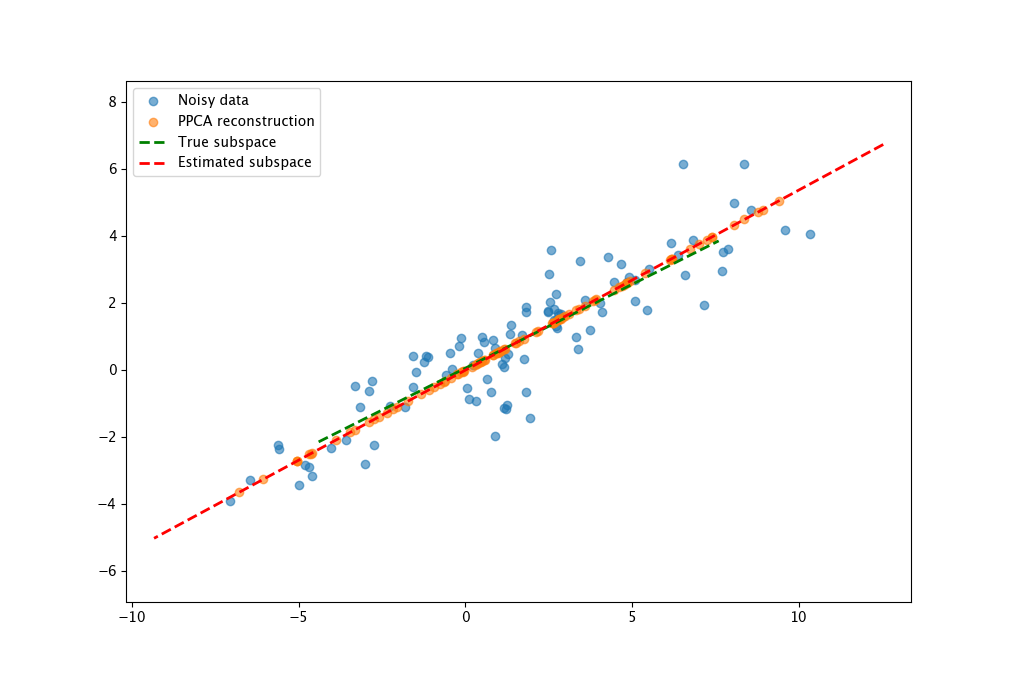
\includegraphics[scale=0.4]{img/ppca_2d.png}
      \caption{Our estimated principal subspace is pretty close to the true subspace.} 
    \end{figure}
  \end{example}

  It turns out that the MLE of $W$ for PPCA, denoted $W_{\mathrm{PPCA}}^\ast = (\Sigma - \sigma^{\ast 2} I_d)^{1/2} V_k$ has columns in the same direction but with a smaller length than $W_{\mathrm{PCA}} = S V_k = \Sigma^{1/2} V_k$ for standard PCA. For this reason, you should think of PPCA as ``almost'' PCA. In fact, let's demonstrate this with a quick code example. 

  \begin{example}[PPCA vs PCA]
    We fit PPCA and PCA onto the same dataset. 
    \begin{lstlisting}
      import numpy as np
      import matplotlib.pyplot as plt
      from mpl_toolkits.mplot3d import Axes3D

      np.random.seed(42)
      n = 150
      z1 = np.random.normal(0, 1, n)
      z2 = np.random.normal(0, 1, n)
      z = np.column_stack([z1, z2])
      W_true = np.array([[1, 0.5], [0.8, 1], [0.3, 0.7]])
      mu_true = np.array([1, 2, 0.5])
      X_clean = z @ W_true.T + mu_true
      X = X_clean + np.random.normal(0, 0.3, X_clean.shape)

      # Shared preprocessing
      mu = np.mean(X, axis=0)
      X_centered = X - mu
      Sigma_hat = X_centered.T @ X_centered / n
      eigenvals, V = np.linalg.eigh(Sigma_hat)
      idx = np.argsort(eigenvals)[::-1]
      eigenvals, V = eigenvals[idx], V[:, idx]

      d, k = 3, 2
      V_k = V[:, :k]

      # PPCA
      sigma2_hat = np.sum(eigenvals[k:]) / (d - k)
      Lambda_adjusted = np.maximum(eigenvals[:k] - sigma2_hat, 0)
      W_ppca = V_k @ np.diag(np.sqrt(Lambda_adjusted))

      M = W_ppca.T @ W_ppca + sigma2_hat * np.eye(k)
      z_recon = X_centered @ W_ppca @ np.linalg.inv(M)
      X_ppca_recon = z_recon @ W_ppca.T + mu

      # Regular PCA
      W_pca = V_k @ np.diag(np.sqrt(eigenvals[:k]))
      U, s, Vt = np.linalg.svd(X_centered, full_matrices=False)
      X_pca_recon = U[:, :k] @ np.diag(s[:k]) @ Vt[:k, :] + mu

      # Plotting...
    \end{lstlisting}
    We indeed see that they generate different fits. 

    \noindent\begin{minipage}{.5\textwidth}
      \begin{lstlisting}[]{Code}
        PPCA W matrix:
        [[-1.03970713 -0.34416644]
         [-1.26026994  0.14944401]
         [-0.72131911  0.23497575]]
        Column norms: [1.78593742 0.44271622]
      \end{lstlisting}
      \end{minipage}
      \hfill
      \begin{minipage}{.49\textwidth}
      \begin{lstlisting}[]{Output}
        PCA W matrix:
        [[-1.05394957 -0.41427404]
         [-1.27753377  0.17988615]
         [-0.73120011  0.28284092]]
        Column norms: [1.81040212 0.53289867]
      \end{lstlisting}
    \end{minipage}

    \begin{figure}[H]
      \centering 
      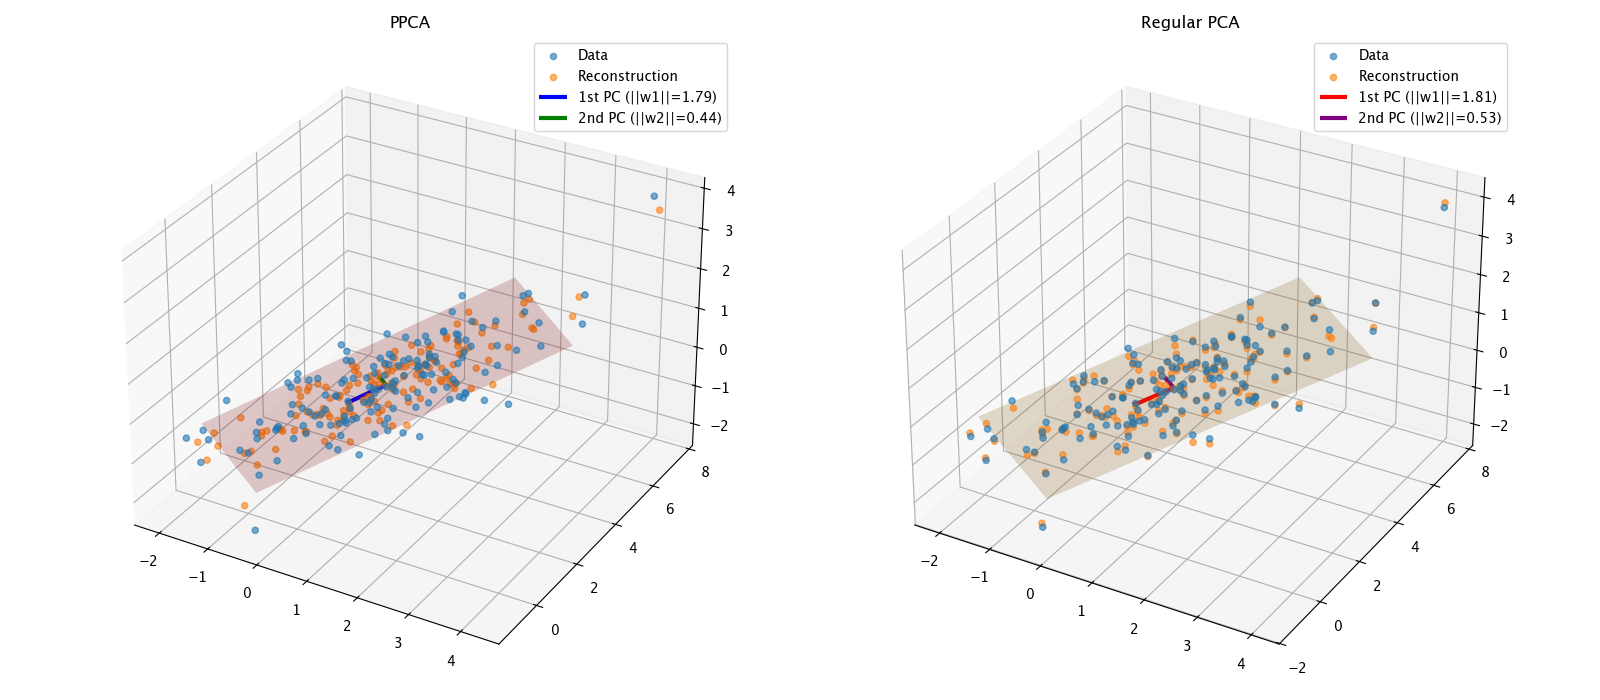
\includegraphics[scale=0.35]{img/ppca_vs_pca.png}
      \caption{The same dataset fitted with PPCA (left) and PCA (right). You can see that their norms are different.} 
    \end{figure}
  \end{example}

  Our next result is intuitive. We have introduced the error term $\epsilon$ that allows us to extend beyond the principal subspace. If we let $\epsilon$ vanish, the density model defined by PPCA becomes very sharp around these $d$ dimensions spanned by the columns of $W$. At $0$, we are reduced to regular PCA. 

  \begin{theorem}[PPCA as $\sigma \to 0$] 
    As $\sigma \rightarrow 0$, the MLE estimates of $W$ is equivalent to that of PCA. That is, when $W \in \mathbb{R}^{d \times k}$, 
    \begin{equation}
      W^\ast = \Sigma V_k
    \end{equation} 
    where $X = U \Sigma V^T$, and $V_k$ is the matrix formed by the first $k$ columns of $V$. That is, the conditional expected value of $z$ given $X$ becomes an orthogonal projection of $X - \mu$ onto the subspace spanned by the columns of $W$. 
  \end{theorem}
  \begin{proof}
    At $0$, our MLE of $W$ is simplified and we have 
    \begin{equation}
      x = W^\ast z + \mu^\ast + \epsilon = \Sigma V_k z + \mu^\ast
    \end{equation}
    which essentially reduces to regular PCA. 
  \end{proof}

  Intuitively, we can see that we are estimating the Gaussian, which corresponds to the mean squared distance from each $x^{(i)}$ to $\ell_k$. 

\subsection{Linear Factor Models} 

  A linear factor model is pretty much the same thing as PPCA. In fact, I don't even know why these two models are distinguished. The only two differences is notation and that linear factor models loosen the restriction that the covariance matrix of $\epsilon$ must be isotopic. 

  \begin{definition}[Linear Gaussian Factor Model] 
    A \textbf{linear Gaussian factor model} is a latent factor model that models the data generating distribution $x$ over $\mathbb{R}^d$ as 
    \begin{equation}
      x = \mu + \Lambda \eta + \epsilon, \eta \sim N(0, I_k), \epsilon \sim N(0, \Psi)
    \end{equation}
    for some diagonal matrix $\Psi$. The parameters are $\theta = \{\Lambda, \mu, \Psi\}$.\footnote{It is also common notation to use $L$ and $f$ as the loading matrix and factors.} $\mu = \mathbb{E}[x]$ simply normalizes the distribution, $\eta \in \mathbb{R}^k$ are the \textbf{factors} that act as latent variables. $\Lambda \in \mathbb{R}^{d \times k}$ is the \textbf{loading matrix} that maps the factors to the samples and $\epsilon$ is an error term. 
    Let's go over the assumptions. 
    \begin{enumerate}
      \item  $\eta$ is $0$-mean (since the translation is captured in $\mu$) and isotropic.\footnote{This parallels the uncorrelated assumptions of PCA and PPCA.}
      \item $\epsilon$ has mean $0$ and has component variables that are uncorrelated, which is reflected in $\Psi$ being diagonal.
      \item $\eta$'s are independent of each other. 
      \item $\epsilon$'s are independent of each other. 
      \item $\epsilon$'s are uncorrelated with $\eta$'s. 
    \end{enumerate}
  \end{definition} 

  The biggest glaring change is really just the terminology. Rather than components, we say \textit{factors}, and rather than projections, we say \textit{loadings}. Finally, we say observable component $x_i$ \textit{loads on} factor $z_j$ if $\Lambda_{ji} \neq 0$, i.e. if $z_j$ affects the value of $x_i$. However, factor models just have more degrees of freedom. In practice, they also perform very similarly, but we will discuss the subtleties soon. 

  To get more comfortable with the notation, let's write out the formula given a data matrix. If we were working with the data matrix $X \in \mathbb{R}^{n \times d}$, then we would be using right matrix multiplication, and so our model will look like 
  \begin{equation}
    X - \mu = \eta \Lambda + \epsilon
  \end{equation}
  where $\eta \in \mathbb{R}^{n \times k}$, $\Lambda \in \mathbb{R}^{k \times d}, \epsilon \in \mathbb{R}^{n \times d}$. 

  \begin{lemma}[Marginal Distribution of Linear Gaussian Factor Model]
    We claim that given $\theta = \{\mu, \Lambda, \Psi\}$, we have
    \begin{equation}
      x \sim \mathcal{N}(\mu, \Lambda \Lambda^T + \Psi)
    \end{equation}
  \end{lemma}
  \begin{proof}
    We know that linear transformations and sums of Gaussians are Gaussian. Therefore, it suffices to compute the mean and variance. For the mean, we have 
    \begin{align}
      \mathbb{E}[x] &= \mathbb{E}[\mu + \Lambda \eta + \epsilon] \\
      &= \mu + \Lambda \mathbb{E}[\eta] + \mathbb{E}[\epsilon] \\
      &= \mu + \Lambda \cdot 0 + 0 \\
      &= \mu
    \end{align}

    For the variance, since $x - \mu = \Lambda \eta +  \epsilon$, 
    \begin{align}
      \text{Var}(x) &= \mathbb{E}[(x - \mu)(x - \mu)^T] \\
      &= \mathbb{E}[(\Lambda \eta + \epsilon)(\Lambda \eta + \epsilon)^T] \\
      &= \mathbb{E}[(\Lambda \eta + \epsilon)(\eta^T \Lambda^T + \epsilon^T)] \\
      &= \mathbb{E}[\Lambda \eta \eta^T \Lambda^T + \Lambda \eta  \epsilon^T + \epsilon \eta^T \Lambda^T + \epsilon \epsilon^T ]
    \end{align}
    
    Since $\eta$ and $\epsilon$ are uncorrelated, we have 
    \begin{align}
      \mathbb{E}[\eta \epsilon^T] &= \mathbb{E}[\eta]\mathbb{E}[\epsilon^T] = 0 \\
      \mathbb{E}[\epsilon \eta^T] &= \mathbb{E}[\epsilon]\mathbb{E}[\eta^T] = 0
    \end{align}
    
    Therefore, the cross terms vanish. 
    \begin{align}
      \text{Var}(x) &= \mathbb{E}[\Lambda \eta \eta^T \Lambda^T] + \mathbb{E}[\epsilon \epsilon^T] \\
      &= \Lambda \mathbb{E}[\eta \eta^T] \Lambda^T + \mathbb{E}[\epsilon \epsilon^T] \\ 
      &= \Lambda I_k \Lambda^T + \Psi \\
      &= \Lambda \Lambda^T + \Psi
    \end{align}
  \end{proof}

  Note that in factor models, we generally do not need the assumption that $\epsilon$ is Gaussian. This is just an extra choice we make in order to compute the marginal distribution. 

  \begin{theorem}[Log-Likelihood and Risk of Linear Gaussian Factor Model]
    The negative log-likelihood---which will act as our loss---of a single sample is 
    \begin{equation}
      L(x \mid \Lambda, \mu, \Psi) = \frac{1}{2} \log|\Lambda \Lambda^T + \Psi| + \frac{1}{2} (x - \mu)^T (\Lambda \Lambda^T + \Psi)^{-1} (x - \mu)
    \end{equation} 
    This allows us to define our risk (expected loss) and therefore our empirical risk/loss for a dataset of $n$ elements $\{x^{(i)}\}_{i=1}^n$. 
    \begin{align}
      R(\Lambda, \mu, \Psi) & = \mathbb{E}_x [ L(x \mid \Lambda, \mu, \Psi)] = \int L(x \mid \Lambda, \mu, \Psi) \, p(x) \,dx \\
      \hat{R}(\Lambda, \mu, \Psi) & = \frac{1}{2n} \sum_{i=1}^n \left[ \frac{p}{2} \log{2 \pi} + \log|\Lambda \Lambda^T + \Psi| + (x^{(i)} - \mu)^T (\Lambda \Lambda^T + \Psi)^{-1} (x^{(i)} - \mu) \right] \\ 
                                  & = \frac{p}{2} \log{2 \pi} + \frac{1}{2} \log|\Lambda \Lambda^T + \Psi| + \frac{1}{2} \text{Tr}\left[(\Lambda \Lambda^T + \Psi)^{-1} \hat{\Sigma}\right]
    \end{align}
    where $\hat{\Sigma} = \frac{1}{n}\sum_{i=1}^n (x^{(i)} - \mu)(x^{(i)} - \mu)^T$ is the sample covariance matrix.\footnote{Notice that the likelihood---and therefore the loss---only involves the data through the sample covariance matrix $\hat{\Sigma}$. The actual factor scores $\eta$ are not needed.}
  \end{theorem}
  \begin{proof}
    From our previous result, we know that the marginal distribution of the observed data is:
    \begin{equation}
      x \sim \mathcal{N}(\mu, \Lambda \Lambda^T + \Psi)
    \end{equation}
    
    The likelihood function is the probability density:
    \begin{equation}
      p(x | \Lambda, \mu, \Psi) = \frac{1}{(2\pi)^{p/2}|\Lambda \Lambda^T + \Psi|^{1/2}} \exp\left(-\frac{1}{2}(x-\mu)^T(\Lambda \Lambda^T + \Psi)^{-1}(x-\mu)\right)
    \end{equation}
    
    Taking the negative log-likelihood to define our loss function:
    \begin{align}
      L(x \mid \Lambda, \mu, \Psi) &= -\log p(x | \Lambda, \mu, \Psi) \\
      &= \frac{p}{2}\log(2\pi) + \frac{1}{2}\log|\Lambda \Lambda^T + \Psi| + \frac{1}{2}(x-\mu)^T(\Lambda \Lambda^T + \Psi)^{-1}(x-\mu)
    \end{align}
    
    Dropping the constant term $\frac{p}{2}\log(2\pi)$ (which doesn't affect optimization), we get:
    \begin{equation}
      L(x \mid \Lambda, \mu, \Psi) = \frac{1}{2} \log|\Lambda \Lambda^T + \Psi| + \frac{1}{2} (x - \mu)^T (\Lambda \Lambda^T + \Psi)^{-1} (x - \mu)
    \end{equation}
    
    The risk is the expected loss over the true data distribution:
    \begin{equation}
      R(\Lambda, \mu, \Psi) = \mathbb{E}_x [L(x \mid \Lambda, \mu, \Psi)] = \int L(x \mid \Lambda, \mu, \Psi) \, p(x) \,dx
    \end{equation}
    
    The empirical risk is the average loss over our dataset. For completeness, let's include back the constant terms. 
    \begin{align}
      \hat{R}(\Lambda, \mu, \Psi) &= \frac{1}{n} \sum_{i=1}^n L(x^{(i)} \mid \Lambda, \mu, \Psi) \\
      &= \frac{1}{n} \sum_{i=1}^n \left[ \frac{p}{2} \log{2 \pi} + \frac{1}{2} \log|\Lambda \Lambda^T + \Psi| + \frac{1}{2} (x^{(i)} - \mu)^T (\Lambda \Lambda^T + \Psi)^{-1} (x^{(i)} - \mu) \right] \\
      &= \frac{p}{2} \log{2 \pi} + \frac{1}{2} \log|\Lambda \Lambda^T + \Psi| + \frac{1}{2n} \sum_{i=1}^n (x^{(i)} - \mu)^T (\Lambda \Lambda^T + \Psi)^{-1} (x^{(i)} - \mu)
    \end{align}

    Now we use a neat trick. The sum on the right is just a scalar, so it is equal to its own trace. Then by using the linearity of trace and the cyclic trace property, we get 
    \begin{align}
      \Tr \left( \sum_{i=1}^n (x^{(i)} - \mu)^T (\Lambda \Lambda^T + \Psi)^{-1} (x^{(i)} - \mu) \right) 
      & = \Tr \left( \sum_{i=1}^n (x^{(i)} - \mu)^T (\Lambda \Lambda^T + \Psi)^{-1} (x^{(i)} - \mu) \right) \\ 
      & = \sum_{i=1}^n \Tr \left( (x^{(i)} - \mu)^T (\Lambda \Lambda^T + \Psi)^{-1} (x^{(i)} - \mu) \right) \\ 
      & = \sum_{i=1}^n \Tr \left( (\Lambda \Lambda^T + \Psi)^{-1} (x^{(i)} - \mu) (x^{(i)} - \mu)^T \right) \\ 
      & = \sum_{i=1}^n \Tr \left( (\Lambda \Lambda^T + \Psi)^{-1} \hat{\Sigma} \right) \\ 
      & = \sum_{i=1}^n \Tr \left( (\Lambda \Lambda^T + \Psi)^{-1} \hat{\Sigma} \right) \\ 
      & = n \Tr \left( (\Lambda \Lambda^T + \Psi)^{-1} \hat{\Sigma} \right)
    \end{align}
    and substituting this back in gives our desired result. 
  \end{proof}

  Unlike PPCA, this empirical loss is not convex, so it must be optimized with numerical methods. In most cases, the solutions tend to be similar, and the MLE estimates between PPCA and FA tend to share the same properties, e.g. the non-uniqueness of $W$ up to rotational factor. 

\subsection{Numerical Solvers for Linear Factor Models}
  
  Since there is not an analytical solution of factor models, much less an analogue of Eckart-Young theorem, we introduce the development of mainstream numerical techniques. 

  \begin{algo}[Iterated Principal Factors]
    \begin{algorithm}[H]
      \caption{Iterated Principal Factors}
      \begin{algorithmic}[1]
        \Procedure{IteratedPrincipalFactors}{$X \in \mathbb{R}^{n \times d}$, $k$}
            
        \Require{Data matrix $X$, number of factors $k < d$}
        \Ensure{Loading matrix $\Lambda \in \mathbb{R}^{d \times k}$, uniquenesses $\Psi \in \mathbb{R}^{d \times d}$}
        
        \State $R \gets \text{corr}(X)$ \Comment{Sample correlation matrix}
        \State $h^2_i \gets 1 - 1/R_{ii}$ for $i = 1, \ldots, d$ \Comment{Initial communalities}
        \State $R^* \gets R$ with $\text{diag}(R^*) = h^2$ \Comment{Reduced correlation matrix}
        \State $\text{converged} \gets \text{False}$
        
        \While{not converged}
          \State $h^2_{\text{old}} \gets h^2$
          \State $V, D \gets \text{eigen}(R^*)$ \Comment{Eigendecomposition}
          \State $\Lambda \gets V_{:,1:k} \sqrt{D_{1:k,1:k}}$ \Comment{First $k$ factors}
          
          \For{$i \gets 1$ to $d$}
            \State $h^2_i \gets \sum_{j=1}^k \Lambda_{ij}^2$ \Comment{Update communalities}
          \EndFor
          
          \State $R^* \gets R$ with $\text{diag}(R^*) = h^2$
          \State $\text{converged} \gets ||h^2 - h^2_{\text{old}}||_2 < \epsilon$
        \EndWhile
        
        \For{$i \gets 1$ to $d$}
          \State $\Psi_{ii} \gets 1 - h^2_i$ \Comment{Uniquenesses}
        \EndFor
        
        \State \Return $\Lambda, \Psi$
        \EndProcedure
      \end{algorithmic}
    \end{algorithm}
  \end{algo}

  \begin{example}[Code Walkthrough]
    In numpy, we can code this up. 

    \begin{lstlisting}
      import numpy as np
      import matplotlib.pyplot as plt
      from scipy.linalg import eigh

      # Generate synthetic data
      np.random.seed(42)
      n = 200  # number of samples
      k = 2    # number of factors
      d = 3    # number of observed variables

      # True parameters
      eta = np.random.randn(n, k)  # factors (isotropic gaussian)
      Lambda_true = np.array([[0.8, 0.3],
                             [0.6, 0.7], 
                             [0.9, 0.2]])  # loading matrix (3x2)

      # Generate noise with different std devs
      noise_std = np.array([0.3, 0.5, 0.2])
      epsilon = np.random.randn(n, d) * noise_std

      # Generate observed data
      X = eta @ Lambda_true.T + epsilon
      X = X - np.mean(X, axis=0)  # center data

      # Iterated Principal Factors Algorithm
      def iterated_principal_factors(X, k, max_iter=1000, tol=1e-6):
         n, d = X.shape
         
         # Compute correlation matrix
         R = np.corrcoef(X.T)
         
         # Initialize communalities
         h2 = 1 - 1/np.diag(R)
         
         for iteration in range(max_iter):
             h2_old = h2.copy()
             
             # Create reduced correlation matrix
             R_star = R.copy()
             np.fill_diagonal(R_star, h2)
             
             # Eigendecomposition
             eigenvals, eigenvecs = eigh(R_star)
             
             # Sort in descending order
             idx = np.argsort(eigenvals)[::-1]
             eigenvals = eigenvals[idx]
             eigenvecs = eigenvecs[:, idx]
             
             # Extract first k factors
             Lambda = eigenvecs[:, :k] @ np.diag(np.sqrt(np.maximum(eigenvals[:k], 0)))
             
             # Update communalities
             h2 = np.sum(Lambda**2, axis=1)
             
             # Check convergence
             if np.linalg.norm(h2 - h2_old) < tol:
                 break
         
         # Compute uniquenesses
         psi = 1 - h2
         
         return Lambda, psi, iteration + 1

      # Fit the model
      Lambda_est, psi_est, iterations = iterated_principal_factors(X, k=2)
    \end{lstlisting}

    It turns out that we get 
    \begin{equation}
      \hat{\Lambda} = \begin{bmatrix}
        -0.959 & 0.051 \\
        -0.708 & -0.167 \\
        -0.946 & 0.073
      \end{bmatrix} \not\approx \begin{bmatrix}
        0.8 & 0.3 \\
        0.6 & 0.7 \\
        0.9 & 0.2
      \end{bmatrix} = \Lambda_{\mathrm{true}}
    \end{equation}
    which is not a good estimate. But remember that factor analysis is invariant to rotations $R$. Though it can find the proper subspace spanned by these two columns (latent variables), it cannot actually converge onto a basis. Therefore, if we carefully choose a rotation matrix $R$,\footnote{This can be done using SVD.} we see that this is indeed a good approximate. 

    \begin{equation}
      \begin{bmatrix}
        0.8 & 0.3 \\
        0.6 & 0.7 \\
        0.9 & 0.2
      \end{bmatrix} \approx 
      \begin{bmatrix}
        -0.959 & 0.051 \\
        -0.708 & -0.167 \\
        -0.946 & 0.073
      \end{bmatrix} 
      \begin{bmatrix}
        -0.909 & -0.418 \\
        0.418 & -0.909
      \end{bmatrix} = \begin{bmatrix}
        0.892 & 0.354 \\
        0.574 & 0.447 \\
        0.890 & 0.329
      \end{bmatrix}
    \end{equation}

    \begin{figure}[H]
      \centering 
      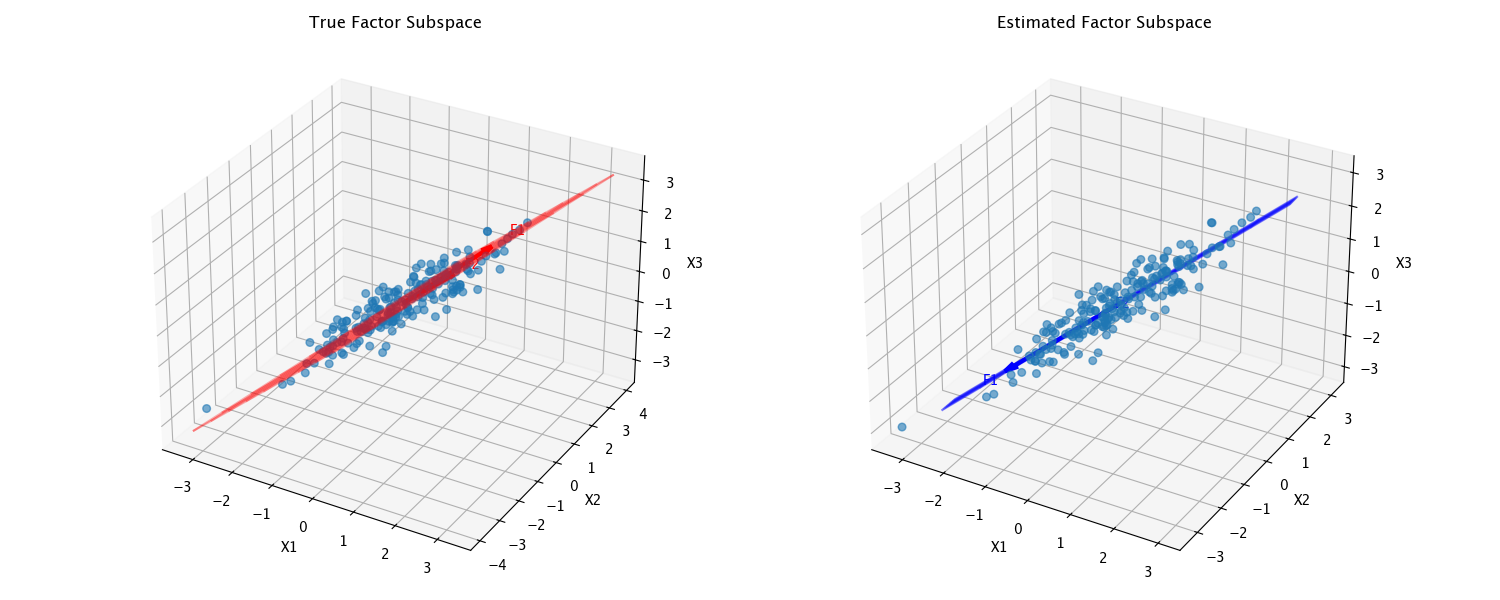
\includegraphics[scale=0.4]{img/factor.png}
      \caption{The subspace spanned by our estimate of the 2-dimensional latent variables (right) does seem like a good approximate to the true subspace (left).} 
    \end{figure}
  \end{example}

\subsection{PCA vs PPCA vs Factor Models} 

  We have stressed that FA is the same as PPCA, but let's get serious and talk about the differences. In a sense, we could have reformulated PCA as a probabilistic model by assuming that the error terms were normally distributed with variance \textit{orthogonal} to the principal subspace. This would have given the exact same expected risk and thus the models would be equivalent. On the other hand, probabilistic PCA assumes an isotropic Gaussian and factor models assume uncorrelated Gaussian. 

  \begin{figure}[H]
    \centering
    \begin{subfigure}[b]{0.6\textwidth}
      \centering
      
\begin{tikzpicture}[scale=1.5]
        % Left: Green diagonal line through cross
        \draw[thick] (-0.8, 0) -- (0.8, 0);  % horizontal
        \draw[thick] (0, -0.8) -- (0, 0.8);  % vertical
        \draw[thick, green!70!black, line width=2pt] (-0.6, -0.6) -- (0.6, 0.6);  % diagonal
        
        % Right: Plus sign and yellow diagonal
        \node at (1.5, 0) {$+$};
        \draw[thick] (2.2, 0) -- (3.8, 0);   % horizontal
        \draw[thick] (3, -0.8) -- (3, 0.8);  % vertical
        \draw[thick, orange!80!yellow, line width=2pt] (2.4, 0.6) -- (3.6, -0.6);  % diagonal
      \end{tikzpicture}
      \caption{Probabilistic interpretation of regular PCA.}
    \end{subfigure}
    
    \begin{subfigure}[b]{0.6\textwidth}
      \centering
      
\begin{tikzpicture}[scale=1.5]
        % Left: Green diagonal line through cross (same as top)
        \draw[thick] (-0.8, 0) -- (0.8, 0);  % horizontal
        \draw[thick] (0, -0.8) -- (0, 0.8);  % vertical
        \draw[thick, green!70!black, line width=2pt] (-0.6, -0.6) -- (0.6, 0.6);  % diagonal
        
        % Right: Plus sign and yellow circle
        \node at (1.5, 0) {$+$};
        \draw[thick] (2.2, 0) -- (3.8, 0);   % horizontal
        \draw[thick] (3, -0.8) -- (3, 0.8);  % vertical
        \draw[thick, orange!80!yellow, line width=2pt] (3, 0) circle (0.5);  % circle
      \end{tikzpicture}
      \caption{Regular interpretation of probabilistic PCA.}
    \end{subfigure}
    
    \begin{subfigure}[b]{0.6\textwidth}
      \centering
      
\begin{tikzpicture}[scale=1.5]
        % Left: Green diagonal line through cross (same as second)
        \draw[thick] (-0.8, 0) -- (0.8, 0);  % horizontal
        \draw[thick] (0, -0.8) -- (0, 0.8);  % vertical
        \draw[thick, green!70!black, line width=2pt] (-0.6, -0.6) -- (0.6, 0.6);  % diagonal
        
        % Right: Plus sign and yellow circle
        \node at (1.5, 0) {$+$};
        \draw[thick] (2.2, 0) -- (3.8, 0);   % horizontal
        \draw[thick] (3, -0.8) -- (3, 0.8);  % vertical
        \draw[thick, orange!80!yellow, line width=2pt] (3, 0) ellipse (0.7 and 0.4);  % ellipsoid
      \end{tikzpicture}
      \caption{Factor analysis.}
    \end{subfigure}
    \caption{The green (left) represents the latent feature, and the orange on the right represents the errors. Figure credits to \textit{ttnphns} from \href{https://stats.stackexchange.com/questions/1576/what-are-the-differences-between-factor-analysis-and-principal-component-analysi}{here}.}
  \end{figure}

  It turns out that this simple change of not having constant variance in the Gaussian error term $\epsilon$ has some implications. 

  \begin{example}[Scaling Features does not Affect FA]
    Remember that in PCA, we must normalize each component of the data to unit variance since PCA tries to maximize variance of projections. However, FA does not chase large-noise features that are uncorrelated with other features. 
  \end{example}

  \begin{example}[FA is Affected by Rotation of Data]
    FA is affected by rotation of the data. \cite{2018schmidt}
  \end{example}

  \begin{theorem}[Factor Models Converge to PPCA in High Dimensions]
    As $d \to +\infty$, factor models are the same model as PPCA. 
  \end{theorem}

